\documentclass{article}


\usepackage{Sweave}

\begin{document}
\input{analysis-concordance}

The following code loads the result file and the file containing the words of the task.

\begin{Schunk}
\begin{Sinput}
> results_raw <- read.csv("~/Documents/Projects/mathesis-is/analysis/results.csv")
> words <- read.csv("~/Documents/Projects/mathesis-is/task/task-src/words.csv")
\end{Sinput}
\end{Schunk}

Now we can merge the result and words files into one single data frame.

\begin{Schunk}
\begin{Sinput}
> results <- merge(results_raw, words, by.x = "word", by.y = "lex")
\end{Sinput}
\end{Schunk}

To check that the duration of each word token as spoken by the participants, we first need to split the data into two subsets: one with monosyllabic words and one with bisyllabic words.

\begin{Schunk}
\begin{Sinput}
> results_mono <- subset(results, syl_no == "mono")
> results_bi <- subset(results, syl_no == "bi")
\end{Sinput}
\end{Schunk}

We can now separately check the duration of monosyllabic and bisyllabic words.

\begin{Schunk}
\begin{Sinput}
> plot(
+     c(), c(),
+     xlim = c(0.1,0.9),
+     ylim = c(0,150),
+     xlab = "duration (s)", ylab = "frequency"
+ )
> hist(
+     results_mono$dur_word, add = TRUE, col = "darkgrey"
+ )
> hist(
+     results_bi$dur_word, add = TRUE, col = "lightgrey"
+ )
\end{Sinput}
\end{Schunk}
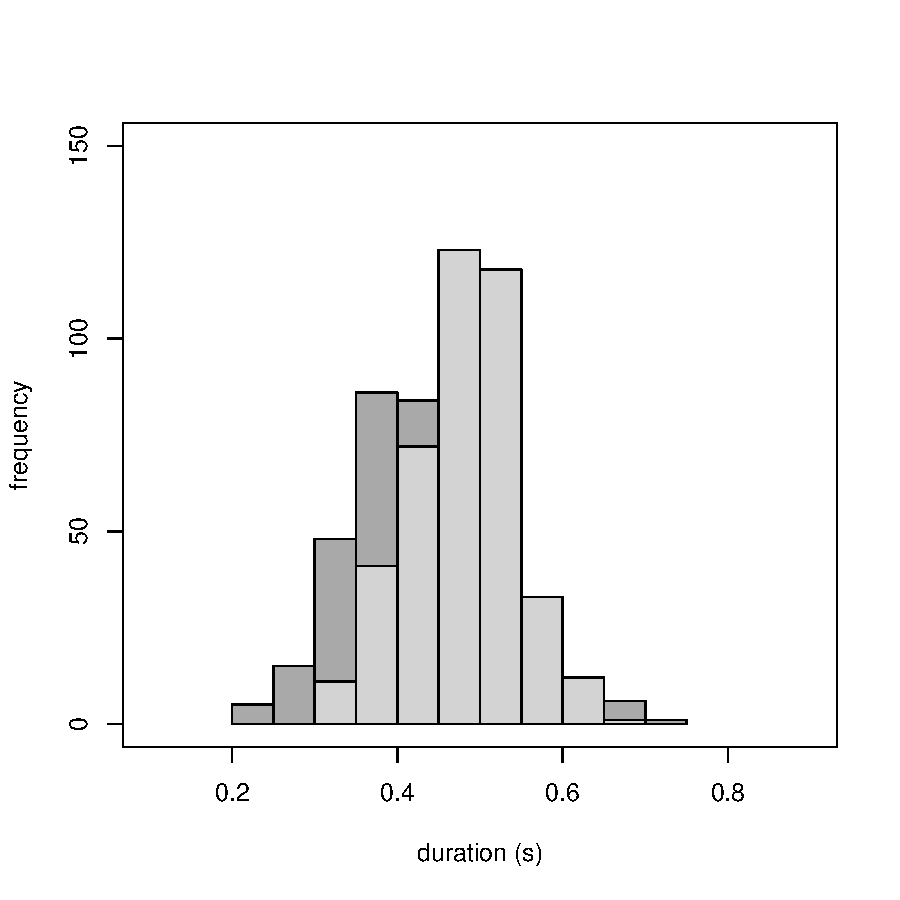
\includegraphics{analysis-004}

The mean length of monosyllabic words is 0.44s, while that of bisyllabic words is 0.48s.

Since I am looking at the duration of the normalised modal voicing of the vocalic gesture, we should first check if there is a significant difference in length of modal voicing between mono- and bisyllabic words.

\begin{Schunk}
\begin{Sinput}
> norm_abs_voic_density <- density(results$norm_abs_voic)
> x.limits <- range(norm_abs_voic_density$x)
> y.limits <- range(norm_abs_voic_density$y)
> plot(
+ c(), c(),
+ xlim = x.limits,
+ ylim = y.limits,
+ xlab = "duration (s)", ylab = "density"
+ )
> lines(density(results_mono$norm_abs_voic), lw = 1, col = "blue")
> lines(density(results_bi$norm_abs_voic), lw = 1, col = "red")
\end{Sinput}
\end{Schunk}

A two-sample unpaired \textit{t}-test shows that the length of modal voicing in words starting with an aspirated stop and ending in a stop is significantly longer in monosyllabic words than in bisyllabic words. Thus, subsequent tests will be performed for monosyllabic and bisyllabic words separately.

\begin{Schunk}
\begin{Sinput}
> results_mono_stop <- subset(results_mono, manner == "stop")
> results_mono_asp_stop <- subset(results_mono_stop, cons1 == "asp")
> results_bi_stop <- subset(results_bi, manner == "stop")
> results_bi_asp_stop <- subset(results_bi_stop, cons1 == "asp")
> t.test(results_mono_asp_stop$norm_abs_voic, results_bi_asp_stop$norm_abs_voic)
\end{Sinput}
\begin{Soutput}
	Welch Two Sample t-test

data:  results_mono_asp_stop$norm_abs_voic and results_bi_asp_stop$norm_abs_voic
t = 4.0716, df = 84.867, p-value = 0.0001044
alternative hypothesis: true difference in means is not equal to 0
95 percent confidence interval:
 0.01317368 0.03831995
sample estimates:
mean of x mean of y 
0.1900476 0.1643007 
\end{Soutput}
\end{Schunk}

\begin{Schunk}
\begin{Sinput}
> results_mono_nasp_stop <- subset(results_mono_stop, cons1 == "nasp")
> results_mono_voi_stop <- subset(results_mono_stop, cons1 == "voi")
> results_mono_vls_stop <- subset(results_mono_stop, cons1 == "vls")
> results_mono_no_stop <- subset(results_mono_stop, cons1 == "no")
> results_bi_nasp_stop <- subset(results_bi_stop, cons1 == "nasp")
\end{Sinput}
\end{Schunk}


\begin{Schunk}
\begin{Sinput}
> norm_abs_voic_density <- density(c(results_mono_asp_stop$norm_abs_voic[results_mono_asp_stop$asp == "yes"],results_mono_asp_stop$norm_abs_voic[results_mono_asp_stop$asp == "yes"]))
> x.limits <- range(norm_abs_voic_density$x)
> y.limits <- range(norm_abs_voic_density$y)
> plot(
+ c(), c(),
+ xlim = x.limits,
+ ylim = y.limits,
+ xlab = "duration (s)", ylab = "density"
+ )
> lines(density(results_mono_asp_stop$norm_abs_voic[results_mono_asp_stop$asp == "yes"]), lw = 1, col = "blue")
> lines(density(results_mono_asp_stop$norm_abs_voic[results_mono_asp_stop$asp == "no"]), lw = 1, col = "red")
\end{Sinput}
\end{Schunk}
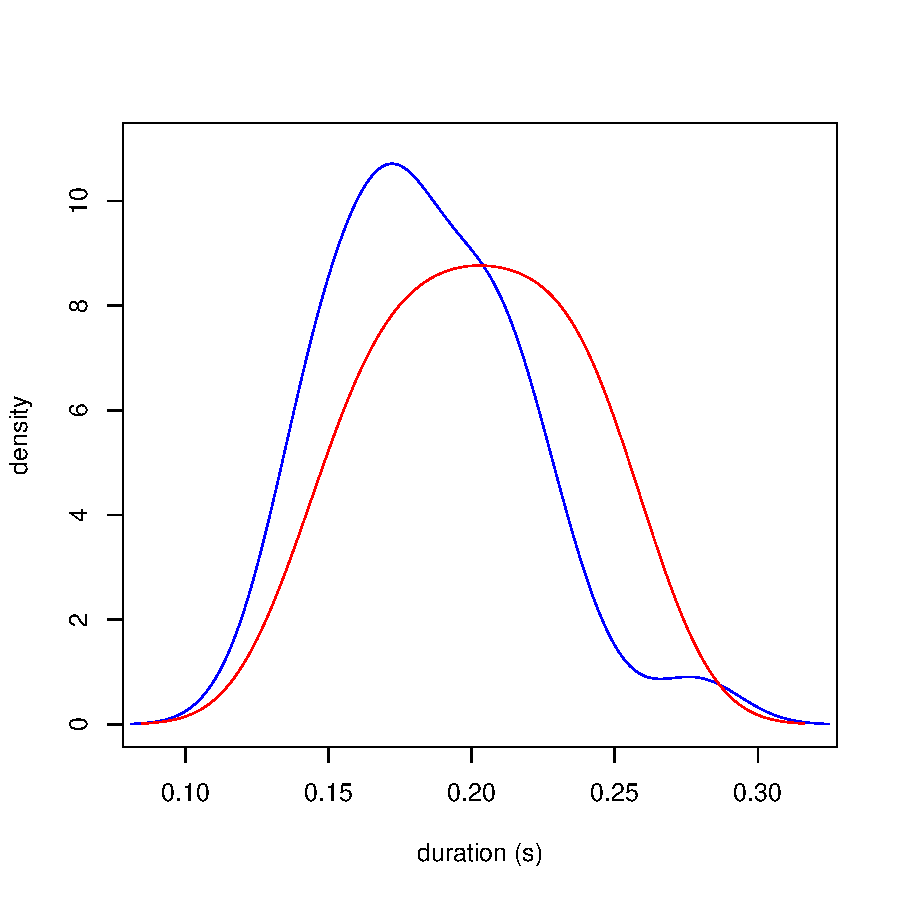
\includegraphics{analysis-008}

\begin{Schunk}
\begin{Sinput}
> shapiro.test(results_mono_asp_stop$norm_abs_voic[results_mono_asp_stop$asp == "yes"])
\end{Sinput}
\begin{Soutput}
	Shapiro-Wilk normality test

data:  results_mono_asp_stop$norm_abs_voic[results_mono_asp_stop$asp ==     "yes"]
W = 0.96782, p-value = 0.4815
\end{Soutput}
\begin{Sinput}
> shapiro.test(results_mono_asp_stop$norm_abs_voic[results_mono_asp_stop$asp == "no"])
\end{Sinput}
\begin{Soutput}
	Shapiro-Wilk normality test

data:  results_mono_asp_stop$norm_abs_voic[results_mono_asp_stop$asp ==     "no"]
W = 0.97906, p-value = 0.9627
\end{Soutput}
\end{Schunk}

Since the distributions of the duration of modal voicing in the two conditions (non-aspirated and pre-aspirated stops) are not significantely different from the normal distribution, I can perform a \textit{t}-test.

\begin{Schunk}
\begin{Sinput}
> boxplot(results_mono_asp_stop$norm_abs_voic~results_mono_asp_stop$asp)
> t.test(results_mono_asp_stop$norm_abs_voic~results_mono_asp_stop$asp)
\end{Sinput}
\begin{Soutput}
	Welch Two Sample t-test

data:  results_mono_asp_stop$norm_abs_voic by results_mono_asp_stop$asp
t = 1.5527, df = 26.893, p-value = 0.1322
alternative hypothesis: true difference in means is not equal to 0
95 percent confidence interval:
 -0.00552171  0.03985344
sample estimates:
 mean in group no mean in group yes 
        0.2014915         0.1843256 
\end{Soutput}
\end{Schunk}
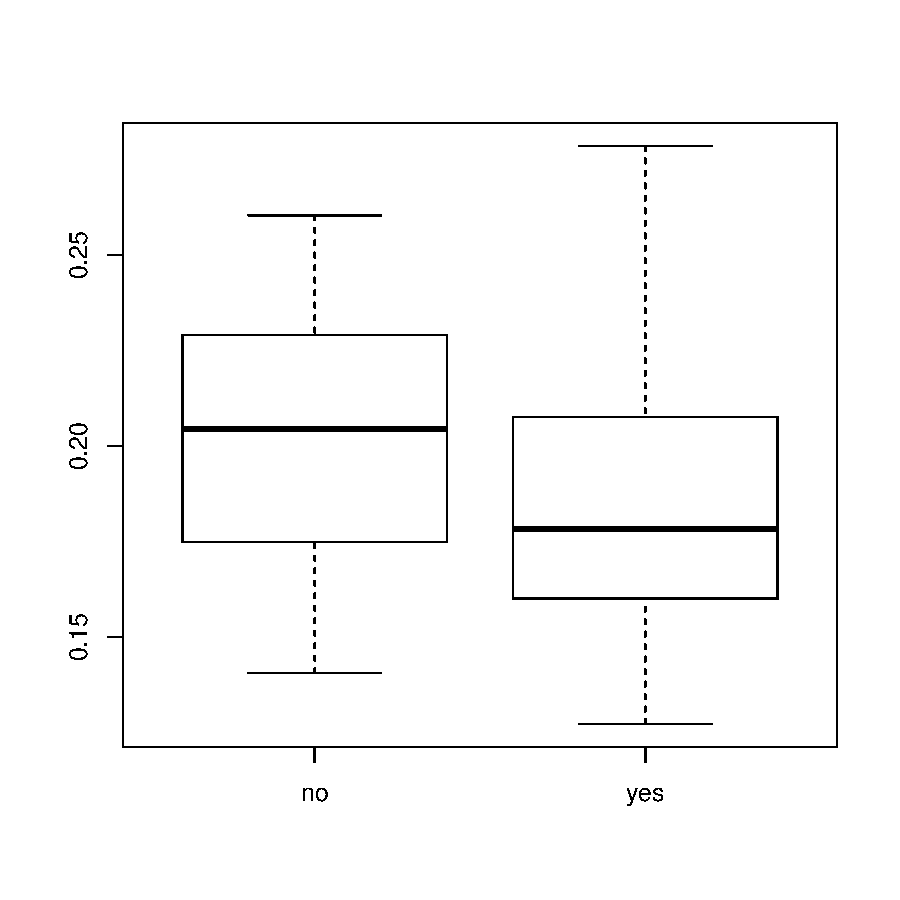
\includegraphics{analysis-010}

\end{document}
